\scanpage{191}
$X$ préschéma connexe, \deleted{\unsure{(réduite, ce qui ne restreint p|réduit, ce qui ne restreint p}}

$1^\circ)$ $X_{\mathrm{réd}}$ de car $p>0$. Alors dans le pro-torseur fondamental $(T_\alpha)$, il n'y a pas en général de sections pour les $T_\alpha$. \deleted{On} On dispose uniquement, \deleted{de façon canonique}

(i) des $\xi_{\ell}^{(\alpha)}\in T_\alpha(\mathbf Z_{\ell})$, $l\ne p$, provenant sans doute de $\xi_{\ell}\in T_\alpha(\widetilde{\mathbf Z}_{\ell\mathbf Z})$
\margin{Coh. $l$-adique}
\margin{hensélisé}

\diagram{\begin{tikzcd}[ampersand replacement=\&,column sep=0pt,row sep=3.3em]
\text{(ii) d'un }\xi_p^{(\alpha)}\in T_\alpha( \& \mathbb{W}_p(k)\arrow[dr,swap,"{\text{``DeRham-Hodge''}}"] \& )\quad\text{si } \deleted{X\ \text{de t.f. sur}}\inserted{\text{$k$ est un}}\ \inserted{\text{corps parfait sur $X$}}\,\deleted{\text{le corps parfait }k} \\
\text{(iii) }\bigl[\,?\quad\text{\uline{réduit}}\ \xi_p^{(\alpha)\,0}\in T_\alpha( \& \deleted{\mathbb{W}}\ \& k\,)\ \bigr]
\end{tikzcd}}
\margin{\figure{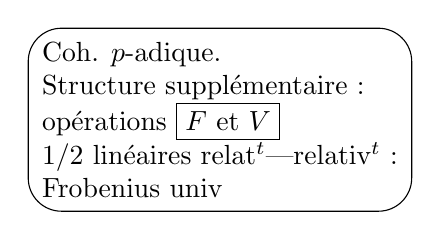
\begin{tikzpicture}
\node[draw,rounded corners=12pt,align=left,inner sep=5pt] {Coh. $p$-adique.\\Structure supplémentaire :\\opérations \fbox{\uuline{$F$} et \uuline{$V$}}\\$1/2$ \uuline{linéaires} \uuline{\unsure{relat$^t$|relativ$^t$}} :\\Frobenius univ};
\end{tikzpicture}}}
\margin{Coh. Hodge-de Rham Mais ici, il faut \deleted{sans doute} donc aller dans la catégorie $\overline{\unsure{M|\mathcal{M}}}$ dérivée. Tenir compte aussi de la structure \uline{filtrée} en Hodge-De Rham}

[$\xi_p$ provenant sans doute d'un $\xi_p\in T_p(\overset{\sim\!\sim}{\mathbf Z}_{p\mathbf Z})$]\margin{hensélisé strict.}

\margin{\unsure{N.B.}}
Si $X=\operatorname{Spec}\mathbf F_q$, il y a en général des \deleted{\unsure{pts}} obstructions non triviales dans des $H^2(\mathbf Q,G)$ \ldots

\deleted{On} On utilise des ``foncteurs fibres'' qui induisent sur les motifs effectifs de poids $0$ le foncteur canonique. Alors les \unsure{objets|d pts} de $T_\alpha(\mathbf Z_\ell)$ sont sans doute uniques \inserted{à isom près}, (th. de Lang), de $=$ ceux de $T_\alpha(\deleted{\unsure{\mathbf Z}}\mathbb{W}_p(k))$ si $k$ fini (id), \inserted{plus gén.} pour un $k$ parfait de dim ch $1$ (?). En général, il faut s'attendre que $T_\alpha(k)$ \deleted{soit un} ait plus d'un élément à isom près, mais il est possible que $T_{\deleted{\unsure{\alpha|\infty}}}(k)=\varprojlim T_\alpha(k)$ n'a qu'un élément à isom près, celui donné par la théorie de DeRham-Hodge.
\margin{relation avec les problèmes galoisiens ?? Il doit être \uline{équivalent}, cf \uline{Manin}}
\margin{190}
